\documentclass{article}
\usepackage{hyperref}
\usepackage[utf8]{inputenc}
\usepackage{graphicx}
\usepackage{geometry}
 \geometry{
	 a4paper,
	 total={170mm,257mm},
	 left=20mm,
 	top=20mm,
 } 
 
\title{EPI-USE: IoT-Homecare \\
The Inevitables
}

\author{  
            Peter Rayner\\
            Dawie Pritchard\\
            Drew Langley\\
            Hendrik Jan van der Merwe\\
            Lyle Nel\\
        }


\begin{document}

\maketitle

\includegraphics[width=20cm,height=11cm,keepaspectratio]{group.JPG}

\newpage

\tableofcontents

\newpage


\section{High level description}
A home care system that takes advantage of the Internet of Things. The system will make use of existing devices and sensors to deliver a holistic system for monitoring homecare patients.The system will gather details from a patient from the devices and sensors and communicate them in a generic manner using Wi-Fi with the caregivers through a mobile application and EPI-USE's cloud server (EPI-USE IoT Homecare pdf.2017) 

\subsection{Possible Project Name}
Intellicare

\newpage
\section{Proposed Solution}

\subsection{Technologies}
\begin{itemize}
	\item J2EE
	\item JDBC
	\item JPA
	\item Wildfly 10
	\item GlassFish 4
\end{itemize}

\subsection{Deployment Diagram}
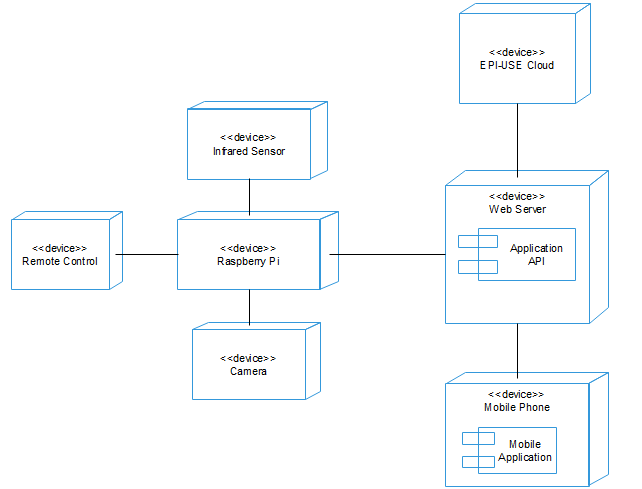
\includegraphics[width=20cm,height=11cm,keepaspectratio]{DeploymentDiagram.png} \\

\subsubsection{Description}
We intend to primarily make use of three types of devices that will be used for the system. These devices will use the Raspberry Pi as a communication device between the webserver containing the application API and the EPI-USE cloud where data will be stored. This will ensure that if the Raspberry Pi breaks or is under certain circumstances rendered inoperable that it be the only loss and that no important data be lost along with it. A mobile application will also be developed for use by the caretaker. This application will gather information and alert care givers if there is an emergency. We will be using a microservices architecture where each microservice can be managed, developed and released independently. \\ \\ \\The devices that will be used are:\\ \\
\textbf{Infrared Sensors} \\
There are two ways in which we intend to use these sensors. The first being a sensor triggered light beneath the bed. When a person gets up from the bed at night a light mounted beneath the bed will be switched on. Giving the person enough light to move around safely. This is to address the problem of elderly and disabled people falling down at night while trying to move around their living space. The next way we intend to use this technology is using these sensors to detect when a person is falling down the stairs and to notify the caregivers when this happens. \\ \\
\textbf{Remote Control} \\
A remote control device is to be used by the patient select which meal they would like to eat along with what they want to drink. This information can be used to derive the likes and dislikes of a patient and assist the caregivers in understanding what the patient likes and dislikes. \\ \\
\textbf{Cameras} \\
Cameras are to be used in case of an emergency. If a patient falls down or if an event occurs that might register as an emergency, an alarm can be triggered and the caregivers are alerted, thus allowing them to observe the patients by means of a camera and determine whether there is in fact an emergency and act upon it.

\newpage
\section{Development Methodology}
We will be using the Agile Scrum Methodology. By making a backlog of work to be done and by completing deadlines in short iterations or sprints. We will meet daily by making use of  Slack Messaging Platform to discuss the progress as well as obstacles and how to overcome these obstacles by getting input from each member. We will also define when these deadlines are and make sure we keep to the schedule. We will meet everytime we are done with a deadline to reflect on the work done. \\ \\
At each deadline or meeting we will make sure we meet with the client to make sure that they are kept up to date with our progress. We will also meet with the client when there are concerns or obstacles to overcome to make sure the client knows  about these obstacles. The client will be kept up to date each week with the progress of the project.

\section{Risk Analysis}
\subsection{Privacy}
The Protection of Personal Information Act, No 4 of 2013, is applicable in this project due to data collection of personal information. We caution that due diligence be exercised when deploying the system withing a home. The act requires that the data subject gives consent or in the case of a patient with dementia, that the guardian of the patient gives consent for data collection. Compliance with the act has additional implications for security, custody of the collected data and how it may be processed.

\subsection{Security}
There are security concerns regarding the use of cameras and sensors involved. Precautions will have to be taken to ensure that patients information and access to these cameras and sensors are limited to only those who require access.


\newpage
\section{Team Details}
\subsection{Dawie Pritchard}
\textbf{Skills:}
\begin{itemize}
 	\item Human Computer Interaction
 	\item Trends, Visual Design 
 	\item Multimedia Specialist
 	\item Computer Scientist
\end {itemize}
\textbf{Technologies known:}
\begin{itemize}
	\item C
 	\item C++
 	\item C\#
 	\item CSS
 	\item Bootstrap
 	\item Java
 	\item Python
 	\item Javascript / AngularJS / ExpressJS / NodeJS / JQUERY
 	\item MongoDB / NoSQL
 	\item PHP
 	\item SQL
 	\item HTML5
 	\item XML
 \end{itemize}
\textbf{Stengths:} 
\begin{itemize}
	\item Front-End
	\item Back-End development
\end{itemize}

\newpage
\subsection {Peter Rayner}

\textbf{Front-end developer with knowledge of:}
\begin{itemize}
 	\item Artifical Intelligence
 	\item Data structures 
 	\item Website design 
 	\item Databases and human computer interaction(user experience)
 \end{itemize}
\textbf{Technologies known:}
\begin{itemize}
	\item C++ 
	\item C 
	\item C\# 
	\item Java 
	\item PHP
	\item MySQL
	\item PostgreSQL
	\item JavaScript 
	\item Python 
	\item Assembly 
	\item AngularJS  
	\item Bootstrap
 \end{itemize}
\textbf{Previous industry experience:}\\
Working at Barclays CIB in big data and analytics.
\\
\newpage
\subsection {Hendrik Jan van der Merwe} 
\textbf{University level knowledge of:}
\begin{itemize}
 	\item Data structures
 	\item Databases
 	\item Human Computer Interaction focussing on User Experience
 	\item System Design
\end{itemize}
\textbf{Technologies known:}
\begin{itemize}
	\item C++
	\item C\#
	\item Java
	\item SQL / MySQL
	\item MongoDB
	\item PHP
	\item JavaScript / AJAX / JQuery / NodeJS / ExpressJS
	\item HTML / CSS / Bootstrap
	\item XML
\end{itemize}
\textbf{Strengths:}
\begin{itemize}
	\item Database Design
	\item Back-end Development
\end{itemize}

\newpage
\subsection {Lyle Nel}
\textbf{Qualifications:} \\

I hold a BTEC in software engineering, which included project management as part of the curriculum.
I also hold a BSc in Computer Systems from Heriot Watt University in Edinburgh, Scotland, with relevant subjects such as Software Engineering, Operations management, Knowledge management, Professional development, and Artificial intelligence.\\ \\
\textbf{Digital electronics:} \\
I have worked with Atmel and ARM microprocessors as well as on the arduino platform. In addition I am familiar with most of the common components of digital circuits including 7400 series and 4000 series integrated circuits. \\ \\
\textbf{Computer Hardware:} \\
I am familiar with all standard consumer hardware and some server hardware. I maintain my own server cluster at home for running experiments. \\ \\
\textbf{Artificial intelligence} \\
I am most experienced in genetic algorithms and I am the author of an open source project that cracks passwords using genetic algorithms. The repository was one of the top 3 trending projects on Github and Hackernews a while back. See https://github.com/lyle-nel/siga. In general I am very comfortable with solving problems within the domain of AI. \\ \\
\textbf{Languages} \\
C, C++ including the new C++11, C++14 and C++17 ISO standards, Bash, Python, Javascript, HTML5, PHP, MSSQL, MySQL, Java, Lisp, Prolog and 64-bit intel assembly. The language that I am most comfortable with is C++. When I conduct experiments on large datasets I use a mixture between C++, Python and Bash. \\ \\
\textbf{Platforms} \\
I do all of my work in a Linux environment.

\newpage
\subsection {Drew Langley}
Third year BIS Multimedia student with experience in UX and HCI, animation and 3D modelling, Web design and databases as well as proficiency in programming. I am currently studying Networks, Software Engineering and Artificial Intelligence. \\ \\
\textbf{Technologies known:}
\begin{itemize}
	\item HTML
	\item CSS 
	\item JS / AngularJS / NodeJS / JQuery 
	\item PHP 
	\item SQL
	\item MongoDB
	\item Java 
	\item C++ 
	\item C 
	\item C\# 
	\item Python 
	\item Assembly
\end{itemize}
\textbf{Experience:} \\
Designed and developed www.ugandaprohunts.com
\\ \\
\textbf{Strengths:} 
\begin{itemize}
	\item Front-End
	\item Back-End development
\end{itemize}

\newpage
\section{Why Choose Us?}
	We believe we are the best team to implement this project as we have all the relevant skills necessary spread throughout our team members to perform above and beyond the call to create the best system possible in terms of functionality, quality, performance and aesthetic appeal. Our skills are split well between technical expertise and back-end/front-end developers.\\ \\
	Our team is also very interested in the ways in which we can collaborate to build such an interesting system, made from so many abstracted parts and features, and ultimately be used to change peoples daily lives for the better.\\ \\
	We are dedicated to performing well as a group and we hope with your collaboration we will be able to provide you with a product which we both can be proud of and can make a difference. \\ \\
    We hope to hear from you soon and look forward to working with you.

\end{document}
